\chapter{Grafische Darstellung von Daten -- Die MatPlotLib}
\label{chp:Matplotlib}
\epigraph{
	Real life seems to have no plots.
}{Ivy Compton-Burnett}

Menschen sind unheimlich gut darin, Bilder zu interpretieren. Computer haben ihre Stärke in der Auswertung von rohen Zahlen. Um nun die Früchte unserer Datenverarbeitung mit Python zu ernten, wollen wir Daten als graphische Plots ausgeben. Ein einfach zu bedienendes Mittel hierzu ist die MatPlotLib bzw. das Untermodul PyPlot. Das Modul MatPlotLib bietet tatsächlich so viele Funktionen, dass damit ein eigenständiger Kurs gefüllt werden könnte. Hier soll Ihnen eine Basis gezeigt werden, mit der Sie die häufigsten Aufgaben lösen können, und auf der Sie im Selbststudium leicht aufbauen können.

Eine erste Übersicht über die Funktionen der MatPlotLib finden Sie auch unter \url{https://matplotlib.org/tutorials/introductory/pyplot.html}.

\section{Grundlagen}
An dieser Stelle möchte ich Ihnen zuerst einen einfachen Code zeigen, und diesen dann Zeile für Zeile \enquote{entziffern}:

\begin{codebox}[Beispiel: Einfacher Plot, width=.55\linewidth, nobeforeafter, equal height group = grpXmpSimplePlot]
\begin{minted}[linenos]{python3}
import math
import matplotlib.pyplot as plt

N = 100
X = [(x - N/2) / 10 for x in range(N)]
Y = [math.sin(x) for x in X]

plt.plot(X, Y)
plt.show()
\end{minted}
\end{codebox}
%
\begin{tcolorbox}[title=Ausgabe: Einfacher Plot, width=.45\linewidth, nobeforeafter, equal height group = grpXmpSimplePlot]
	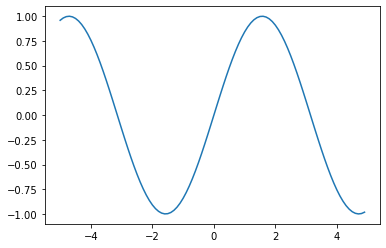
\includegraphics[width=\linewidth]{./gfx/plt-sin}
	\captionof{figure}{Einfacher Plot der matplotlib}
\end{tcolorbox}

In den Zeilen 1 und 2 laden wir Module -- zum einen das Modul \inPy{math}, mit dem wir die Daten generieren, die auf unserem Plot erscheinen sollen, und zum anderen die Matplotlib. Tatsächlich handelt es sich dabei um ein extrem umfangreiches Paket, weswegen wir nur einen Teil davon in unser Projekt integrieren: Das Untermodul \inPy{pyplot}\footnote{Die Matplotlib enthält Code zum Fenstermanagement, zur Interpolation von Kurven, Umgang mit Dateien, ... Alle diese Features bilden den Unterbau von \inPy{pyplot}, müssen aber nicht \enquote{offengelegt} werden, um für uns nützlich zu sein. Während \inPy{pyplot} intern alle diese Objekte und Funktionen benutzt und korrekt verwaltet, können wir uns auf das \emph{Interface} konzentrieren, das uns \inPy{pyplot} auf all diese Features bietet.}. Da dieser Modulname \inPy{matplotlib.pyplot} eher unhandlich ist, hat es sich eingebürgert, \inPy{plt} als Kurzname hierfür zu verwenden.

In den kommenden drei Zeilen generieren wir Werte, die schließlich geplottet werden sollen. \inPy{X} und \inPy{Y} sind jeweils Listen mit \inPy{N = 100} Elementen. Die Werte in \inPy{X} sind einfach gleichverteilte Werte im Abstand von \texttt{0.1}, rund um die \texttt{0} herum. Die Werte in \inPy{Y} enthalten jeweils den Sinus dieser \inPy{X}-Werte. Bis hierhin also haben wir noch nichts Neues gesehen.

In Zeile 8 wird nun die Funktion \inPy{plot} aus dem Modul \inPy{plt} aufgerufen. Diese Funktion bereitet alles vor, das nötig ist, um einen Plot zu generieren: Ein Arbeitsfenster, Achsen mit Beschriftung, Datenpunkte in den Graphen eintragen, ... All das wird aber nur im Arbeitsspeicher vorbereitet, jedoch noch nicht sichtbar gemacht. Grund hierfür ist, dass wir die Standard-Einstellungen noch abändern könnten: eine andere Linienfarbe, Skalierung, Bemaßung, \ldots Wenn jede Änderung in Echtzeit auf dem Bildschirm umgesetzt würde, hätte dies ein unangenehmes Flackern zur Folge, bevor der Plot endlich fertig aufgebaut ist. Stattdessen müssen wir manuell festlegen, wann unser Plot fertig beschrieben ist, \ie wann er auf dem Bildschirm erscheinen soll. Dies geschieht in Zeile 10.

Im einfachsten Fall müssen wir also folgende Arbeitsschritte erledigen:
\begin{itemize}
\item Das Modul \texttt{matplotlib.pyplot} laden
\item X- und Y-Werte als getrennte Listen vorbereiten
\item Die Funktion \texttt{plot} aufrufen
\item Die Funktion \texttt{show} aufrufen
\end{itemize}

Tatsächlich ist das Vorbereiten von X-Werten \emph{streng genommen} sogar überflüssig:

\begin{codebox}[Beispiel: Einfacher Plot ohne X-Werte, width=.55\linewidth, nobeforeafter, equal height group = grpXmpSimplePlotSansX]
\begin{minted}[linenos]{python3}
import matplotlib.pyplot as plt

N = 100
Y = [(x - 50) * x for x in range(N)]

plt.plot(Y)
plt.show()
\end{minted}
\end{codebox}
%
\begin{tcolorbox}[title=Ausgabe: Einfacher Plot ohne X-Werte, width=.45\linewidth, nobeforeafter, equal height group = grpXmpSimplePlotSansX]
	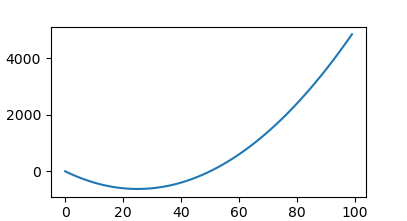
\includegraphics[width=\linewidth]{./gfx/plt-square}
	\captionof{figure}{Einfacher Plot ohne explizite x-Werte}
\end{tcolorbox}

Wenn keine X-Werte angegeben werden, erhalten wir zwar einen \enquote{sinnvollen} Plot; Python hat jedoch natürlich keine Möglichkeit, zu entscheiden, welcher Wert an welche Position gehört. Daher geht der Plotter hier davon aus, dass die Werte bei \inPy{x=0} beginnen und jeweils einen Abstand von \inPy{1} zueinander haben.

Folgen zwei \texttt{plot()}-Befehle direkt aufeinander ohne ein \texttt{show()} dazwischen, so werden beide Graphen auf denselben Plot gezeichnet. Jeder Plot bekommt dabei seine eigene Farbe. Eine Legende wird jedoch nicht \emph{automatisch} angezeigt.

\begin{codebox}[Beispiel: Zwei Graphen im selben Plot, width=.55\linewidth, nobeforeafter, equal height group = grpXmpSimplePlotTwoFunc]
\begin{minted}[linenos]{python3}
import matplotlib.pyplot as plt

N = 100
W = 10
X = [(x - N/2) / W for x in range(N)]
Y = [(x - W/2) * x for x in X]

plt.plot(X, Y)
plt.plot(X, [2 * y for y in Y])

plt.show()
\end{minted}
\end{codebox}
%
\begin{tcolorbox}[title=Ausgabe: Zwei Graphen im selben Plot, width=.45\linewidth, nobeforeafter, equal height group = grpXmpSimplePlotTwoFunc]
	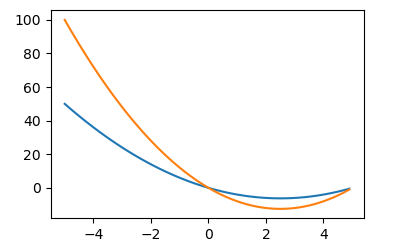
\includegraphics[width=\linewidth]{./gfx/plt-twoFuncs}
	\captionof{figure}{Zwei Graphen}
\end{tcolorbox}

\section{Einfache Formatierungen und andere Plot-Arten}
\subsection{Format-Angaben im Befehl \texttt{plot}}
Es wurde schon angesprochen, dass die Standard-Einstellungen der MatPlotLib nicht übernommen werden müssen. Im einfachsten Fall können wir direkt im \texttt{plot}-Befehl eine andere Linienfarbe und -form festlegen: Nach den Y-Werten kann ein optionaler String übergeben werden, in dem diese Information enthalten ist:
\mint{python3}{plt.plot(X, Y, "r--")}
weist die MatPlotLib dazu an, den Plot in Rot mit Strichlinien zu zeichnen. Dagegen steht
\mint{python3}{plt.plot(X, Y, "b-.")}
für einen Graphen aus blauen Punkten, die durch mit einer Linie verbunden sind. Folgende Zeichen werden verstanden und können auch miteinander kombiniert werden:

\begin{tcolorbox}[title=Format-Strings für \texttt{plt.plot()}]
\textbf{Punktarten}
\vspace{-6pt}
\begin{center}
	\begin{tabular}{cc|cc|cc}
		Symbol     & Punkt         & Symbol                    & Punkt            & Symbol     & Punkt            \tabcrlf
		\texttt{,} & Pixel         & \texttt{.}                & kleiner Punkt    & \texttt{o} & großer Punkt     \\
		\texttt{s} & Quadrat       & \texttt{d}                & schmale Raute    & \texttt{D} & breite Raute     \\
		\texttt{p} & Fünfeck       & \texttt{h}                & Sechseck stehend & \texttt{H} & Sechseck liegend \\
		\texttt{|} & Strich        & \texttt{+}                & Plus             & \texttt{x} & Kreuz            \\
		\texttt{<} & Dreieck links & \texttt{>}                & Dreieck rechts   & \texttt{*} & Stern            \\
		\texttt{v} & Dreieck unten & \texttt{\textasciicircum} & Dreieck oben                                     \\
	\end{tabular}
\end{center}

\textbf{Linienarten}
\vspace{-15pt}
\begin{center}
	\begin{tabular}{cc|cc|cc|cc}
		Symbol     & Linie        & Symbol      & Linie       & Symbol     & Linie     & Symbol      & Linie       \tabcrlf
		\texttt{-} & durchgezogen & \texttt{--} & gestrichelt & \texttt{:} & gepunktet & \texttt{-.} & strichpunkt \\
	\end{tabular}
\end{center}
\end{tcolorbox}
%
\begin{tcolorbox}
\textbf{Farben}
\begin{center}
	\begin{tabular}{cc|cc|cc|cc}
		Symbol     & Farbe   & Symbol     & Farbe   & Symbol     & Farbe & Symbol     & Farbe  \tabcrlf
		\texttt{b} & blau    & \texttt{c} & cyan    & \texttt{g} & grün  & \texttt{k} & schwarz \\
		\texttt{m} & magenta & \texttt{r} & rot     & \texttt{y} & gelb  & \texttt{w} & weiß    \\
	\end{tabular}
\end{center}

\captionof{table}{Formatstring-Elemente für \texttt{plot}}
\label{tab:PlotFormatStrings}
\end{tcolorbox}

Soll eine Kurve in einer Farbe gezeichnet werden, die nicht in Tabelle \ref{tab:PlotFormatStrings} aufgeführt sind, kann das Keyword-Argument \texttt{color} verwendet werden. Hier gibt man die Farbe als RGBA-String mit führendem Raute-Symbol an. Das bedeutet, dass der Rot- Grün- und Blau-Anteil der Farbe sowie die Deckkraft (\enquote{Alpha-Wert}) als zweistellige Hexadezimalzahl geschrieben wird und diese vier Zahlen dann aneinander gereiht werden. Für ein dunkles Rot kann man also schreiben:
\mint{python3}{plt.plot(X, Y, color="#7F0000FF")}
Dabei ist \inPy{7F} der Rot-Anteil (entspricht 50\% Intensität), \inPy{00} jeweils der Grün- und Blau-Anteil und \inPy{FF} die Deckkraft (entspricht 100\%).

\subsection{Legenden Anzeigen und Gitter anzeigen -- \texttt{legend}, \texttt{label} und \texttt{grid}}
Weiter ist es natürlich auch möglich, Graphen zu benennen und eine Legende anzeigen zu lassen. Dazu sind zwei Dinge nötig:
\begin{itemize}
\item Im Plot-Befehl muss mit dem Keyword-Argument \texttt{label} ein Titel angegeben werden
\item Mit dem Befehl \texttt{legend()} muss die Legende auch angezeigt werden:
\end{itemize}

\begin{codebox}[Beispiel: Plot mit Legende, width=.55\linewidth, nobeforeafter, equal height group = grpXmpSimplePlotLegend]
\begin{minted}[linenos]{python3}
import math
import matplotlib.pyplot as plt

N  = 100
X  = [(x - N/2) / 10 for x in range(N)]
Y1 = [math.sin(x) for x in X]
Y2 = [math.cos(x) for x in X]

plt.plot(X, Y1, label="Sinus")
plt.plot(X, Y2, label="Cosinus")

plt.legend()
plt.show()
\end{minted}
\end{codebox}
%
\begin{tcolorbox}[title=Ausgabe: Plot mit Legende, width=.45\linewidth, nobeforeafter, equal height group = grpXmpSimplePlotLegend]
	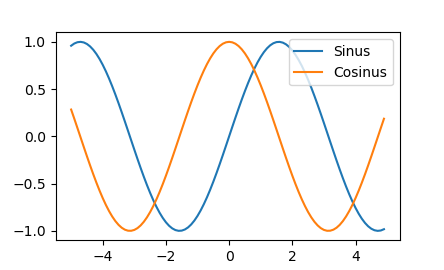
\includegraphics[width=\linewidth]{./gfx/plt-legend}
	\captionof{figure}{Plot mit Legende}
\end{tcolorbox}

Dem Befehl \texttt{plot} können noch viele weitere Keyword-Arguments mitgegeben werden, auf die hier nicht weiter eingegangen werden kann. Sie können sich bei Bedarf selbst die Bedeutung und Anwendung dieser Schlüsselworte anlesen; siehe hierzu die Dokumentation unter 
\url{https://matplotlib.org/2.1.2/api/_as_gen/matplotlib.pyplot.plot.html}

Um die Werte aus dem Plot besser ablesbar zu machen können auch Hilfslinien dazugeschalten werden. Dies erreicht der Befehl \texttt{grid}:

\begin{codebox}[Beispiel: Plot mit Gitterlinien, width=.55\linewidth, nobeforeafter, equal height group = grpXmpSimplePlotGrid]
\begin{minted}[linenos]{python3}
import math
import matplotlib.pyplot as plt

N  = 100
X  = [(x - N/2) / 10 for x in range(N)]
Y1 = [math.sin(x) for x in X]
Y2 = [math.cos(x) for x in X]

plt.plot(X, Y1, label="Sinus")
plt.plot(X, Y2, label="Cosinus")

plt.grid()

plt.legend()
plt.show()
\end{minted}
\end{codebox}
%
\begin{tcolorbox}[title=Ausgabe: Plot mit Gitterlinien, width=.45\linewidth, nobeforeafter, equal height group = grpXmpSimplePlotGrid]
	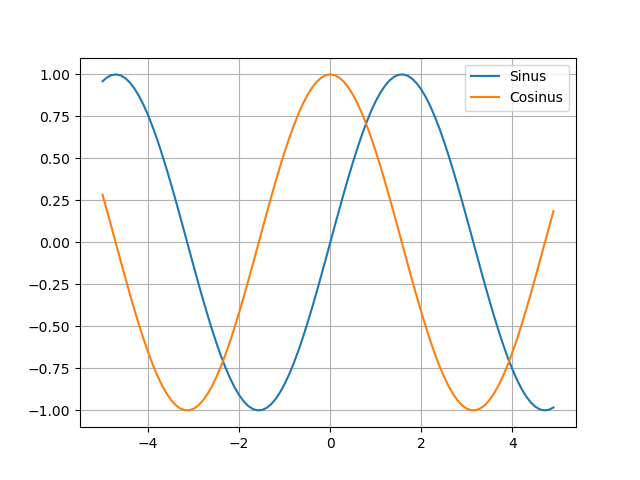
\includegraphics[width=\linewidth]{./gfx/plt-grid}
	\captionof{figure}{Plot mit Gitterlinien}
\end{tcolorbox}

\subsection{Titel und Achsenbeschriftung hinzufügen -- \texttt{title}, \texttt{xlabel}, \texttt{ylabel}}
Neben einer Legende sollten bei Plots auch Titel und Achsenbeschreibungen nicht fehlen. Diese lassen sich einfach über die Befehle \texttt{title}, \texttt{xlabel} und \texttt{ylabel} hinzugefügt werden. Das folgende Beispiel illustriert dies anhand der \emph{spektralen Strahlungsdichte eines idealen schwarzen Körpers}
\footnote{Crash-Kurs Physik:\\
Jeder Körper strahlt elektromagnetische Strahlung aus -- in einfachen Worten, jeder Körper leuchtet. Die Intensität und Lichtfarbe sind von der Temperatur abhängig. Heiße Körper glühen daher rot, sehr heiße Körper kommen sogar bis zur Weißglut; bei \enquote{kühlen} \SI{37}{\celsius} \enquote{leuchten} wir Menschen nur im Infrarot-Bereich. Aus diesem Grund sehen wir zwar nicht immer die Strahlung, die von jedem Körper ausgestrahlt wird, können diese aber trotzdem messen. Das gezeigte Programm berechnet die Intensität der einzelnen Licht-Wellenlängen, die ein Körper mit einer gegebenen Temperatur \texttt{T} ausstrahlt.\\
Streng genommen spielt hierbei auch die Farbe des Körpers eine Rolle; daher sprechen PhysikerInnen auch von \emph{Schwarzkörperstrahlung}. In der Praxis ist dieser Zusammenhang oft vernachlässigbar. Sekunden-Thermometer und Wärmebildkameras funktionieren nach diesem Prinzip: Ein Bild im Infraroten wird vom Objekt aufgenommen; die \enquote{Farbe} der gemessenen Strahlung wird dann als Temperatur interpretiert. Im gezeigten Plot liegt das Strahlungs-Maximum bei ca. \SI{20}{THz}, was einer Wellenlänge von \SI{15}{\micro\meter} entspricht -- weit außerhalb des Rahmens menschlicher Wahrnehmung, die zwischen ca. 400 und \SI{800}{\nano\meter} stattfindet, und damit in Übereinstimmung mit der täglichen Wahrnehmung, dass wir unsere Mitmenschen nicht glühen sehen.\\
Wenn Sie in Zeile 5 den Wert für \texttt{T} auf \inPy{5700} ändern und in Zeile 12 den Plot-Bereich auf \inPy{1e+15} erweitern, wird Ihnen das Spektrum der Sonne mit Maximum im sichtbaren Licht dargestellt.}:

\begin{codebox}[Beispiel: Plot mit Titel und Labels]
\begin{minted}[linenos]{python3}
import math
import matplotlib.pyplot as plt

h  = 6.62607015e-34     # Planck constant
T  = 300                # temperature in Kelvin
c  = 299792458          # speed of light
kB = 1.380649e-23       # Boltzmann constant

spectralDensity = lambda nu : ((2 * h * nu**3) / (c**2))  / \
                              (math.exp((h * nu) / (kB * T)) - 1)
\end{minted}
\end{codebox}
%
\begin{codebox}[]
\begin{minted}[linenos, firstnumber=last]{python3}
X = [x for x in range(1, int(1e+14), int(1e+10))]
Y = [spectralDensity(x) for x in X]

plt.title("Schwarzkörperstrahlung")
plt.xlabel("Strahlungsfrequenz in Hz")
plt.ylabel("Intensität in W/m²")

plt.plot(X, Y)
plt.show()
\end{minted}
\end{codebox}
%
\begin{tcolorbox}[title=Ausgabe: Plot mit Titel und Labels]
	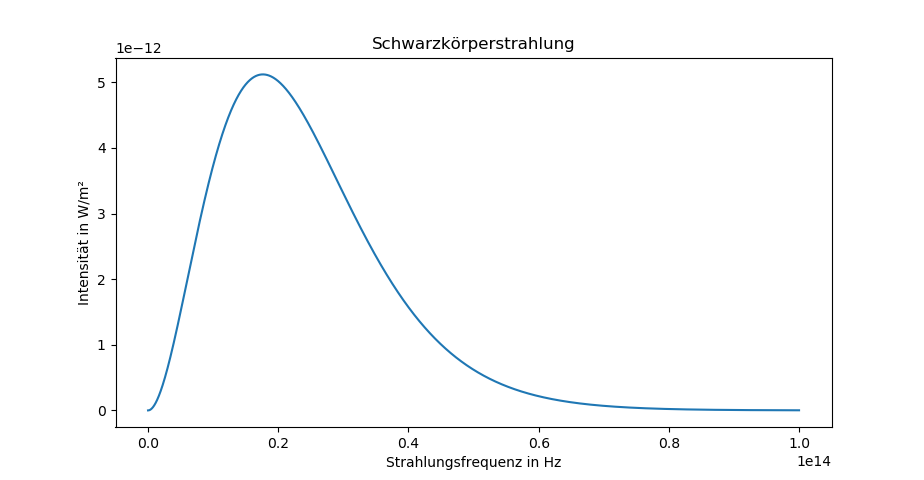
\includegraphics[width=\linewidth]{./gfx/plt-labels}
	\captionof{figure}{Plot mit Titel und Achsenbeschriftungen}
\end{tcolorbox}

\subsection{Skalierung der Achsen -- \texttt{xscale}, \texttt{yscale} und \texttt{xlim}, \texttt{ylim}}
Wenn Plots einen großen Wertebereich abdecken, kann es sinnvoll sein, die Werte \emph{logarithmisch} aufzutragen. Eine oder mehrere Achsen werden dabei verzerrt, um über mehrere Größenordnungen hinweg Änderungen gut zu verfolgen. Hierzu dienen die Befehle \texttt{xscale} und \texttt{yscale}.

\begin{codebox}[Beispiel: Linearer und Logarithmischer Plot]
\begin{minted}[linenos]{python3}
import matplotlib.pyplot as plt

W  = 500
X  = [x / 10 for x in range(-W, W)]
Y1 = [2 ** x for x in X]
Y2 = [x ** 7 for x in X]
\end{minted}
\end{codebox}
%
\begin{codebox}[]
\begin{minted}[linenos, firstnumber=last]{python3}
plt.title("Linear Plot")
plt.plot(X, Y1, label="exponential")
plt.plot(X, Y2, label="power")
plt.legend()
plt.show()

plt.title("Logarithmic Plot")
plt.yscale("log")
plt.plot(X, Y1, label="exponential")
plt.plot(X, Y2, label="power")
plt.legend()
plt.show()
\end{minted}
\end{codebox}

\begin{tcbraster}[raster columns=2,
                  raster equal height,
                  nobeforeafter,
                  raster column skip=0.5cm]
\begin{tcolorbox}[title=Lineare Auftragung]
	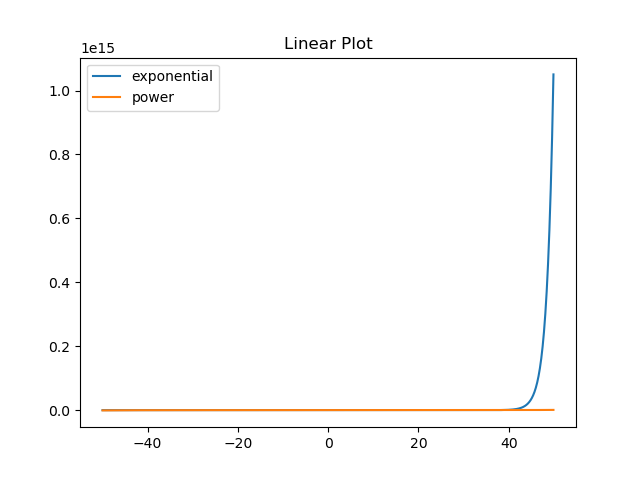
\includegraphics[width=\linewidth]{./gfx/plt-linear}
	\captionof{figure}{Linearer Plot}
	\label{gfx:PlotLinear}
\end{tcolorbox}
%
\begin{tcolorbox}[title=Logarithmische Auftragung]
	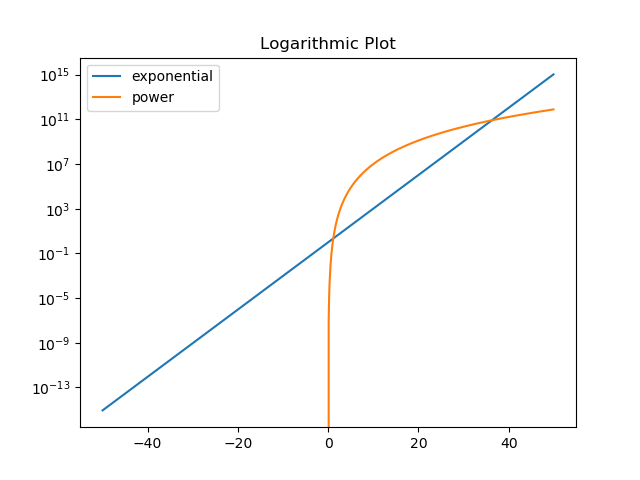
\includegraphics[width=\linewidth]{./gfx/plt-logarithmic}
	\captionof{figure}{Logarithmischer Plot}
	\label{gfx:PlotLogarithmic}
\end{tcolorbox}
\end{tcbraster}

In Abbildung \ref{gfx:PlotLinear} können wir kaum Details erkennen: Beide Plots bleiben \enquote{nahe} an der Null, bis die Exponentialfunktion irgendwann \enquote{explodiert}. Erst bei der logarithmischen Auftragung (Abbildung \ref{gfx:PlotLogarithmic}) sehen wir, dass das Polynom (orange Linie) zeitweise sogar größer ist als die Exponentialfunktion.

Wir haben diese Verzerrung erreicht, indem wir in Zeile 19 die y-Achse logarithmisch skaliert haben. Ebenso könnten wir mit \inPy{plt.xscale("log")} auch die x-Achse verzerren.

Der Logarithmus von 0 oder negativen Werten ist nicht definiert\footnote{liebe MathematikerInnen: natürlich beziehe ich mich auf den reellwertigen Logarithmus bzw. auf den Hauptzweig des Logarithmus.}. Um dennoch mit Werten umzugehen, die das Vorzeichen wechseln können und aber sinnvoller logarithmisch aufgetragen werden sollten, existiert auch die Option \inPy{"symlog"}. Hier wird jeweils der Logarithmus \emph{des Betrags} der Werte aufgetragen; abhängig vom Vorzeichen geschieht dies dann nach oben oder unten (\inPy{plt.yscale("simlog")} bzw. nach links oder rechts (\inPy{plt.xscale("simlog")}. Werte nahe der 0 werden linear aufgetragen. Was als nahe der 0 gelten soll, kann mit den Keyword-Arguments \texttt{linthreshx} bzw. \texttt{linthreshy} bestimmt werden. Die Grenzen des linearen bereichs sind auch als Hilfslinien sichtbar, wenn \texttt{grid} benutzt wird.

Für statistische Auswertungen ist manchmal auch der \enquote{Logit} einer Wahrscheinlichkeit interessant ($\text{logit}(y) = \log(\frac{y}{1-y})$). Für y-Werte zwischen 0 und 1 kann so auch \inPy{plt.xscale("logit")} eingestellt werden.

\begin{codebox}[Beispiel: Auftragung mit \texttt{symlog}]
\begin{minted}[linenos]{python3}
import math
import matplotlib.pyplot as plt

W  = 500
X  = [x / 10 for x in range(-W, W)]
Y1 = [math.sin(x) for x in X]
Y2 = [x / 10      for x in X]

plt.xscale("symlog")
plt.plot(X, Y1)
plt.plot(X, Y2)
plt.grid()
plt.show()

plt.xscale("symlog", linthreshx=10)
plt.plot(X, Y1)
plt.plot(X, Y2)
plt.grid()
plt.show()
\end{minted}
\end{codebox}

\begin{tcolorbox}[title=Auftragung mit \texttt{symlog}]
	\begin{minipage}{.49\linewidth}
		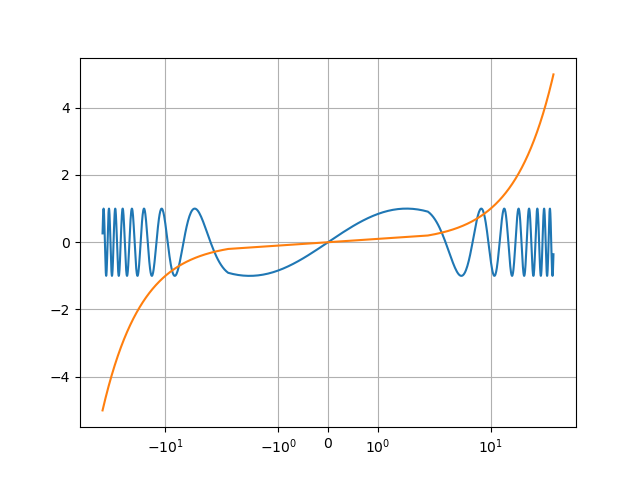
\includegraphics[width=\linewidth]{./gfx/plt-symlog}
		\captionof{figure}{symmetrisch-logarithmische Auftragung mit Standard-Schranke für lineare Auftragung}
		\label{gfx:PlotSymlog}
	\end{minipage}
%
	\begin{minipage}{.49\linewidth}
		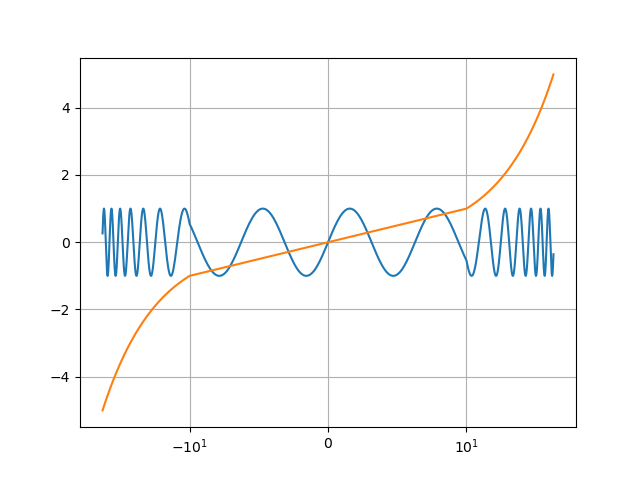
\includegraphics[width=\linewidth]{./gfx/plt-symlog-threshold}
		\captionof{figure}{symmetrisch-logarithmische Auftragung mit höherer Schranke für lineare Auftragung}
		\label{gfx:PlotSymlog-Threshold}
	\end{minipage}
\end{tcolorbox}

In Ähnlicher Manier kann mit \texttt{xlim} und \texttt{ylim} festgelegt werden, in welchen Grenzen die X- und Y-Achse skaliert werden sollen, unabhängig von den \enquote{Ausmaßen} des tatsächlichen Graphen. Der Graph füllt dann nicht mehr die gesamte Plot-Fläche aus, bzw. wird gegebenenfalls abgeschnitten:

\begin{codebox}[Beispiel: Manuell gewählte Plot-Skalierung, width=.55\linewidth, nobeforeafter, equal height group = grpXmpSimplePlotScale]
\begin{minted}[linenos]{python3}
import math
import matplotlib.pyplot as plt

N = 100
X = [(x - N/2) / 10 for x in range(N)]
Y = [math.sin(x) for x in X]

plt.plot(X, Y)
plt.xlim(-6  , +6)
plt.ylim(-0.7, +3)
plt.grid()
plt.show()
\end{minted}
\end{codebox}
%
\begin{tcolorbox}[title=Manuell gewählte Plot-Skalierung, width=.45\linewidth, nobeforeafter, equal height group = grpXmpSimplePlotScale]
	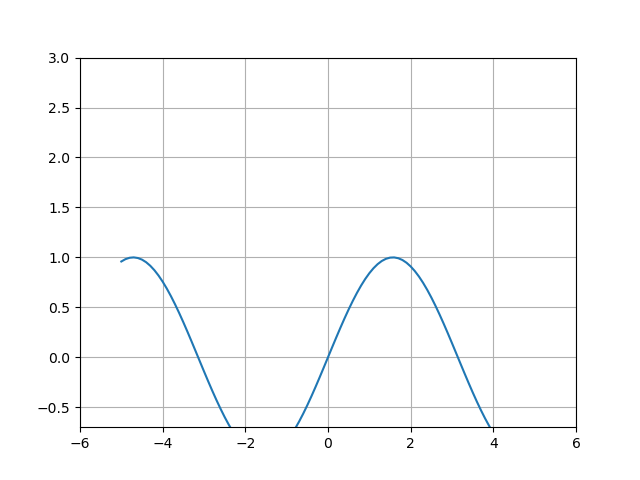
\includegraphics[width=\linewidth]{./gfx/plt-limits}
	\captionof{figure}{Manuelle Skalierung}
\end{tcolorbox}

\subsection{Andere Plot-Arten}
Neben Kurven in einem X-Y-Diagramm kann die MatPlotLib auch andere Arten von Visualisierungen erzeugen.

\subsubsection{Barplots}
Barplots oder Balkendiagramme verhalten sich ähnlich wie die Punkt- oder Liniendiagramme, die im letzten Abschnitt gezeigt wurden. Alle oben erwähnten Befehle funktionieren auch hier, außerdem kann auch das Keyword-Argument \texttt{color} verwendet werden. Erstellt werden Barplots mit den Befehlen \texttt{bar} (vertikale Balken) und \texttt{barh} (horizontale Balken). Die \enquote{X-Werte} dürfen für Barplots auch Strings enthalten, und werden entsprechend als Beschriftung angebracht.

\begin{codebox}[Beispiel: Barplots]
\begin{minted}[linenos]{python3}
import random
import matplotlib.pyplot as plt

X = ["Smoot", "Fnord", "R'lyeh"]
Y = [random.randint(0, 11) for x in X]   # this one goes up to eleven

plt.bar(X, Y, color="#0040B0FF")
plt.ylim(0, 11)
plt.show()

plt.barh(X, Y, color="#0040B0FF")
plt.xlim(0, 11)
plt.show()
\end{minted}
\end{codebox}
%
\begin{tcbraster}[raster columns=2,
                  raster equal height,
                  nobeforeafter,
                  raster column skip=0.5cm]
\begin{tcolorbox}[title=Vertikaler Barplot]
	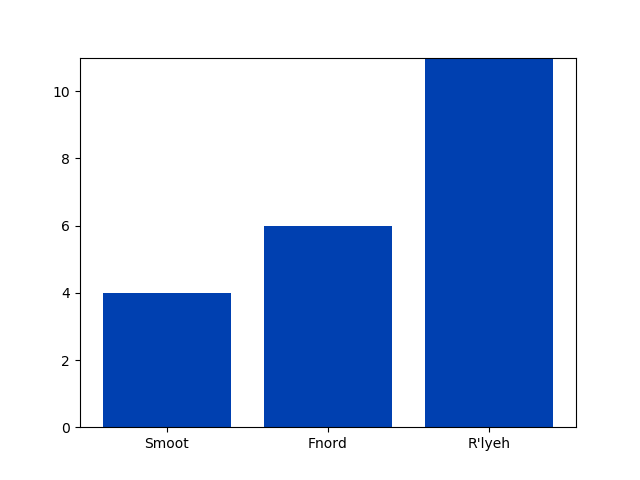
\includegraphics[width=\linewidth]{./gfx/plt-bars}
	\captionof{figure}{Vertikaler Barplot}
\end{tcolorbox}
%
\begin{tcolorbox}[title=Horizontaler Barplot]
	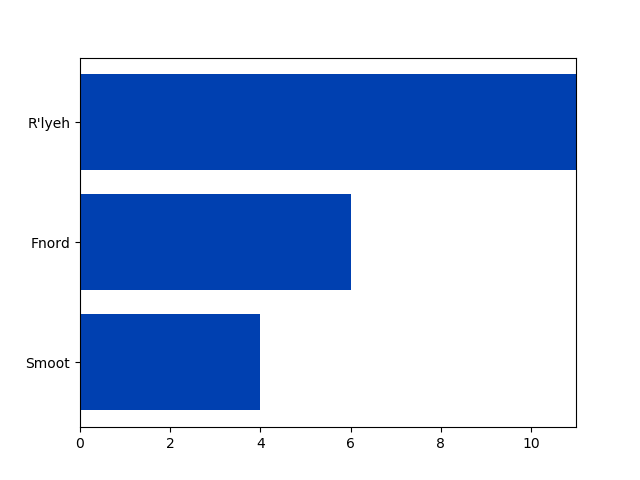
\includegraphics[width=\linewidth]{./gfx/plt-barh}
	\captionof{figure}{Horizontaler Barplot}
\end{tcolorbox}
\end{tcbraster}

\subsubsection{Kuchendiagramme}
pie
\subsubsection{Histogramme}
hist(data, bins, orientation='horizontal')
\subsubsection{Stackplots}
stackplot
\subsubsection{Scatterplots}
scatter
\subsubsection{Flussdiagramme}
quiver
\subsubsection{Äquipotentiallinien}
isosurface

\subsubsection{Weitere Diagrammtypen}
Unter \url{https://matplotlib.org/3.1.0/gallery/index.html} sind diverse Beispiele zum Umgang mit der MatPlotLib aufgeführt.


\section{Multiplots}
subplots

\section{Plot-Objekte}

\section{Ausgabe in Dateien}





%https://matplotlib.org/api/pyplot_api.html


save files, hintbox on data usage